\section{Implementation}


The \pdht system implements a distributed key/value store within a
distributed memory computing cluster. \pdht provides both {\em put}
and {\em get} operations that use a hash function to map an arbitrary
key value to a processor rank and 64-bit hash value, giving each key a
unique location within the distributed hash table.

Each hash table is treated as a distributed array of objects, with a
fixed number of elements per process. Upon the creation of a new
distributed hash table, \pdht creates two new portal table
entries. The first PTE contains the {\em pending} match list and the
second is for the {\em active} match list. The pending match list is
populated with a number of entries that match any incoming
communication requests (i.e. a wildcard). Each ME in the pending list
corresponds to a single entry in the local portion of the distributed
array.

The principal idea in \pdht is to create a match list entry (ME) for
every element in the hash table. The 64-bit hash value produced by the
hash function is used as the value for the match bits field to be used
with the Portals communication requests. By using the hash value as
the match bits field, much of the handling of a get operation can be
relegated to the Portals implementation, which should in turn rely on
network hardware offload when available.

\begin{figure}[ht]
  \centering
  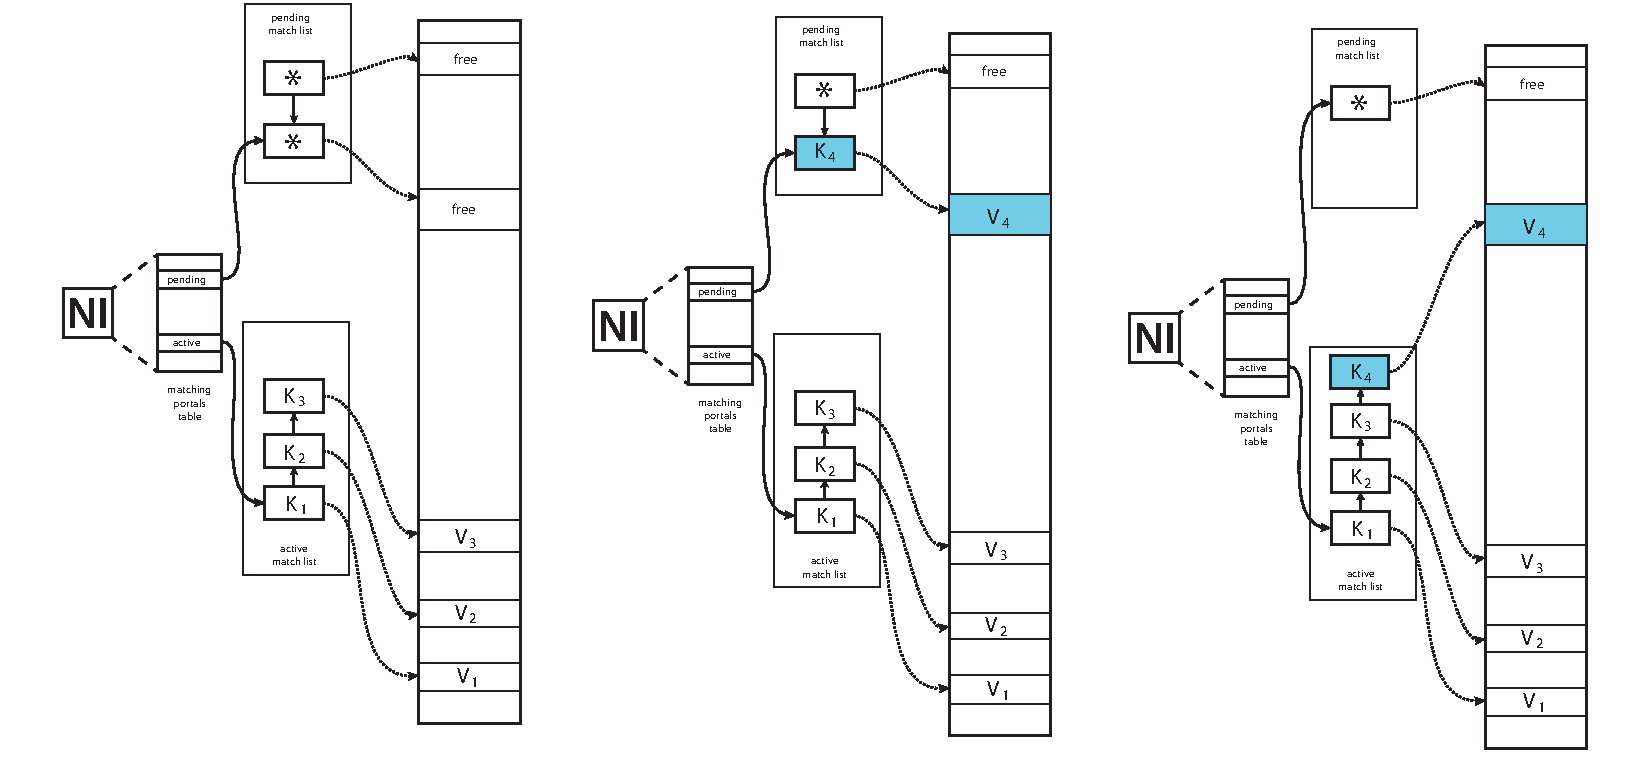
\includegraphics[scale=.35]{figs/put}
  \caption{Slow motion {\tt put()} operation}
  \label{fig:put}
\end{figure}


\subsection{Put Operation}

When adding a new key/value object to the hash table, the key is
hashed, giving both the target processor rank as well as the match
bits field to be used for the entry. In the case of a local insertion,
the initating process can copy the entry into the hash table array and
locally insert a new ME with the match bits set to the hashed value. 

When the entry hashes to a remote process, the initiating process
performs a one-sided put operation onto the pending PTE, consuming one
of the wildcard ME entries on the match list. The hash entry is
transferred and stored into the array entry that is associated with
the pending entry. As shown in Figure \ref{fig:put} (b), at this point
the table entry data resides in the correct location on the target
process, the match lists are in an incomplete state.  To complete the
operation, a new wildcard ME must replace the consumed entry on the
pending list. Additionally, the active list must be updated with an ME
that contains the hash. These actions would result in the state shown
in Figure \ref{fig:put} (c).

The current approach to handle the match list management between the
pending and active lists is to use a dedicated progress thread. This
thread blocks on the event queue associated with the pending PTE,
waiting for incoming put requests. As put requests are received, the
polling thread replaces the consumed wildcard ME and allocates a
new entry in the array for a new object. The thread also creates a new
ME with the appropriate match bits set and appends it to the active
list. Subsequent get operations will find a match in the active list.

\subsection{Get Operation}

Get operations are handled by computing the hash function on the key,
then performing one-sided get request, using the process rank and
match bits provided by the hash. If the get operation is unable to
find a matching entry on the active match list, the operation reports
a not-found message. If the retrieved table entry doesn't match the
requested full key, \pdht notes the collision and either returns
control to the application or performs a linear probe, depending on
the desired behavior.

\subsection{Collisions and Key Sparsity}

In the case that multiple keys map to the same rank/hash pair (a
collision), PDHT utilizes a linear probing solution. The library can
also be configured to simply detect collisions and let the application
take appropriate action. 

A significant difference between traditional hash tables and \pdht is
that using the Portals match list for table entries detaches the link
between the computed hash code and the actual location in
memory. Typically, a hashed key, $K$,  is used with modular arithmetic to
determine a location in an array of size $N$. The hash function is a
provides a mapping between $|K| \rightarrow N$ elements. When $|K|$ is
much larger than $N$, the likelihood of collisions increases.

In \pdht, an array is still used to hold the collection of hash table
entries, but the indexing into this array is performed indirectly,
through the ME in the match list. A \pdht hash function provides the 
mapping: $|K| \rightarrow P \times 2^{64}$. Each key is mapped to one
of $P$ distinct process ranks and a unique 64-bit match bits
value. Compared to traditional implementations, $N \ll  P \times
2^{64}$, which has the impact of dramatically reducing the likelihood
of a collsion, provided a reasonable hash function.


%%% Local Variables:
%%% mode: latex
%%% TeX-master: "paper"
%%% End:
